%----------------------------------------------------------------------------------------
%	PACKAGES AND OTHER DOCUMENT CONFIGURATIONS
%----------------------------------------------------------------------------------------

\documentclass[final]{beamer}

\usepackage[framemethod=TikZ]{mdframed}
\usepackage[scale=1.24]{beamerposter} % Use the beamerposter package for laying out the poster
\usepackage[percent]{overpic}
\usepackage{amsmath}
\usepackage{amssymb}
\usepackage{gensymb}
\usepackage{color}

\usetheme{confposter} % Use the confposter theme supplied with this template

\setbeamercolor{block title}{fg=ngreen,bg=white} % Colors of the block titles
\setbeamercolor{block body}{fg=black,bg=white} % Colors of the body of blocks
\setbeamercolor{block alerted title}{fg=white,bg=dblue!70} % Colors of the highlighted block titles
\setbeamercolor{block alerted body}{fg=black,bg=dblue!10} % Colors of the body of highlighted blocks

\newlength{\sepwid}
\newlength{\onecolwide}
\newlength{\twocolwide}
\newlength{\threecolwide}
\setlength{\paperwidth}{48in} % A0 width: 46.8in
\setlength{\paperheight}{36in} % A0 height: 33.1in
% \setlength{\paperwidth}{44in} % A0 width: 46.8in
% \setlength{\paperheight}{33in} % A0 height: 33.1in
\setlength{\sepwid}{0.024\paperwidth} % Separation width (white space) between columns
\setlength{\onecolwide}{0.31\paperwidth} % Width of one column
\setlength{\twocolwide}{0.464\paperwidth} % Width of two columns
\setlength{\threecolwide}{0.708\paperwidth} % Width of three columns
\setlength{\topmargin}{-0.5in} % Reduce the top margin size
%-----------------------------------------------------------

\usepackage{graphicx}  % Required for including images

\usepackage{booktabs} % Top and bottom rules for tables

\newcommand{\checkedbox}{\textcolor{dgreen}{$\text{\rlap{$\checkmark$}}\square$}}
\newcommand{\checkbox}{$\square$}
%----------------------------------------------------------------------------------------
%	TITLE SECTION
%----------------------------------------------------------------------------------------

\title{Telescope to test CMS Pixel Phase-II Upgrade ROCs and sensors} % Poster title

\author{Caleb Fangmeier} % Author(s)

\institute{Dept.\ of Physics and Astronomy, Univ.\ of Nebraska \-- Lincoln} % Institution(s)

%----------------------------------------------------------------------------------------

\mdfsetup{skipabove=\topskip,skipbelow=\topskip}
\mdfdefinestyle{exampledefault}{%
  outerlinewidth=0pt,innerlinewidth=0pt,
  outerlinecolor=gray,
  roundcorner=8pt,
  tikzsetting={fill=White,
               fill opacity=0.7},
  backgroundcolor=none
}
\begin{document}

\addtobeamertemplate{block end}{}{\vspace*{2ex}} % White space under blocks
\addtobeamertemplate{block alerted end}{}{\vspace*{2ex}} % White space under highlighted (alert) blocks

\setlength{\belowcaptionskip}{2ex} % White space under figures
\setlength\belowdisplayshortskip{2ex} % White space under equations

\begin{frame}[t] % The whole poster is enclosed in one beamer frame
  \small
  The innermost layer of the CMS Detector at the LHC is the Silicon Pixel Tracker. The current version of the detector has performed well and been critical to the physics program of CMS\@.  However, as the LHC produces higher instantaneous luminosities and higher center-of-mass energies, the detector must be upgraded to accommodate. The Phase-II Upgrade of CMS will replace the entire silicon tracking system.  As part of this upgrade, a new section of the pixel tracker will be added in the so-called ``Very-Forward'' (TODO: $\eta$ range)region of the detector.  This new section of the detector will have different pixel geometries than the current detector, and these new geometries must be accurately characterized.  Therefore, a telescope is being developed for the express purpose of characterizing these sensors so pixel geometry can be optimized before settling on a final design to be placed in CMS\@. The telescope operates by using eight layers of silicon-strip sensors, with the device-under-test placed with four on each side. A charged-particle beam is directed so it passes through both the strip sensors and the device-under-test. Measurements from the telescope are taken to reconstruct individual particle tracks.


\begin{block}{Readout Overview}
  \begin{columns}[t]
    \begin{column}{\paperwidth}
      \begin{figure}
        \centering
        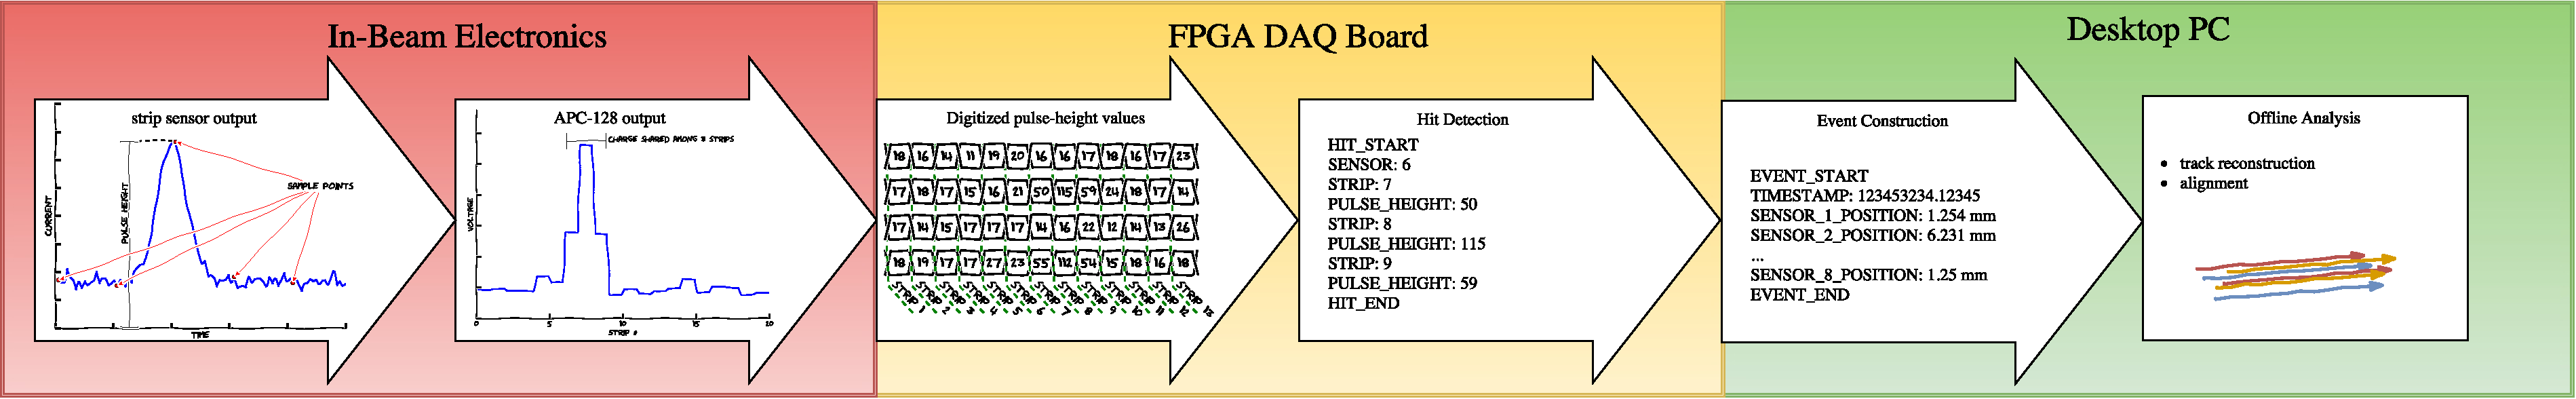
\includegraphics[width=0.98\textwidth]{figures/Telescope_Data_Flow}
      \end{figure}
    \end{column}
  \end{columns}
  \begin{columns}[t]
    \begin{column}{\onecolwide}
      \small
      \begin{itemize}
      \itemsep0em 
        \item The sensor is essentially a silicon NP-Junction operated in ``reverse-bias'' mode where all free charge carriers are evacuated
        \item A energetic charged particle passing through the silicon deposits energy to create free electron-hole pairs which are then separated by the electric field produced by the biasing voltage
        \item The electrons create a current spike that the readout chip, the APC-128, samples and stores
        \item Upon receiving a trigger, the APC-128 serializes the analog pulse-height sample from each of the 128 channels
      \end{itemize}
    \end{column}
    \begin{column}{\onecolwide}
      \small
      \begin{itemize}
      \itemsep0em 
        \item The analog pulse-heights from the 32 APC-128 in the telescope are digitized by 8 high-speed 4-channel ADCs located on the DAQ Board.
        \item The digitized values passed to an FPGA board where they are processed into individual sensor hits.
        \item The sensor hit data is passed across a USB-3 connection to a PC where online software organizes the hits into events and stores them to disk.
      \end{itemize}
    \end{column}
    \begin{column}{\onecolwide}
      \small
      \begin{itemize}
      \itemsep0em 
        \item After the event data is stored to disk, it is ready for offline analysis
        \item Since the detector layers can shift in space significantly, alignment must first be done to accurately measure the geometry of the detector.
        \item After alignment, the various layer hits can be used to construct tracks.
        \item The tracks can then be compared for consistency with the data collected in parallel from the device-under-test.
      \end{itemize}
    \end{column}
  \end{columns}
\end{block}

\begin{columns}[t]
  \begin{column}{\onecolwide}
    \begin{block}{Half-Telescope Sensor Board}
      \centering
      \begin{overpic}[height=20cm]{figures/Half-Telescope-Full}
        \put(5,20){%
          \begin{minipage}{32cm}
            \begin{mdframed}[style=exampledefault]
              \footnotesize
              \begin{itemize}
              \itemsep0em 
                \item Holds 4 strip-sensors with 4 APC-128s each
                \item One sensor board is mounted on each side of the device-under-test
                \item The individual sensor cards can be flipped to rotate the strips 90\degree%
                \item On-board buffers create a low-impedance differential output to transmit the analog pulse-height data via CAT-5 cables to the DAQ board.
                \item Sensor Feature 3
                \item Sensor Feature 4
              \end{itemize}
            \end{mdframed}
          \end{minipage}
          }
      \end{overpic}
    \end{block}
  \end{column}

  \begin{column}{\onecolwide}
    \begin{block}{DAQ Board}
      \centering
      % \begin{overpic}[height=20cm,grid,tics=10]{figures/DAQCard2015_Full_Front}
      \begin{overpic}[height=20cm]{figures/DAQCard2015_Full_Front}
        \put(5,20){%
          \begin{minipage}{29cm}
            \begin{mdframed}[style=exampledefault]
              \footnotesize
              \begin{itemize}
              \itemsep0em 
                \item Supplies the control signals needed by the APC-128s.
                \item 32 ADC Channels to read-out all APC128s in parallel, minimizing dead-time
                \item Incorporates Opal Kelly ZEM4310 (not shown) which features an Altera Cyclone IV FPGA, 128MB of RAM and USB 3
                \item Self-contained power supply circuitry
                \item Handles external triggering, bias-voltage supply, 
              \end{itemize}
            \end{mdframed}
          \end{minipage}
          }
      \end{overpic}
    \end{block}
  \end{column}

  \begin{column}{\onecolwide}
    \begin{alertblock}{Progress}
      \checkedbox System design and parts selection \\
      \checkedbox Circuit design and PCB Layout \\
      \checkbox Assembly and offline testing (in progress)\\
      \checkbox FPGA Firmware development and testing \\
      \checkbox Online/Offline software development \\
      \checkbox Commissioning runs with UNL Diocles electron beam
    \end{alertblock}
    \setbeamercolor{block alerted title}{fg=black,bg=norange} % Change the alert block title colors
    \setbeamercolor{block alerted body}{fg=black,bg=white} % Change the alert block body colors
    \begin{alertblock}{Contact Information}
      \begin{itemize}
      % \item Web: \href{http://www.university.edu/smithlab}{http://www.university.edu/smithlab}
      \item Email: \href{mailto:cfangmeier2@huskers.unl.edu}{cfangmeier2@huskers.unl.edu}
      \item Phone: +1 (402) 768 1358
      \end{itemize}
    \end{alertblock}
  \end{column}
\end{columns}

\begin{columns}[t]
  \begin{column}{2\onecolwide}
    \setbeamercolor{block title}{fg=red,bg=white} % Change the block title color
    \begin{block}{References} 
    \begin{columns}[t]
      \begin{column}{\onecolwide}
        \begin{itemize}
          \item \textbf{PCB Design Files} https://github.com/cfangmeier/VFPIX-telescope-PCB
          \item \textbf{CMS Phase-II Upgrade}
        \end{itemize}
      \end{column}
      \begin{column}{\onecolwide}
        \begin{itemize}
          \item reference 3
          \item reference 4
        \end{itemize}
      \end{column}
    \end{columns}
    \end{block}
  \end{column}
  \begin{column}{\onecolwide}
    \setbeamercolor{block title}{fg=red,bg=white} % Change the block title color
    \small
    \begin{block}{Acknowledgments} 
        Beat Meier \& Tilman Rohe of \textbf{The Paul Scherrer Institute}\\
        Frank Meier of \textbf{Heidelberg University}\\
        Aaron Dominguez \& Rachel Bartek of \textbf{The University of Nebraska \-- Lincoln}
    \end{block}
  \end{column}
\end{columns}

\end{frame} % End of the enclosing frame

\end{document}

